\documentclass[]{report}
\renewcommand\thesection{\arabic{section}} % for page numbering in arabics
\usepackage[utf8]{inputenc}
\usepackage{graphicx,tabularx} % for figures and tables
\usepackage[utf8]{inputenc} % allows special characters such as ä, ö, ỳ
\usepackage[english]{babel} % set the language to English
\usepackage[margin=1.5in]{geometry} % change page margins 
\usepackage{sectsty} % section headers
\subsectionfont{\sffamily\normalsize}
\linespread{1.2} % line distance
\usepackage{lipsum} % http://ctan.org/pkg/lipsum
\usepackage{caption} % use for captions on tables
% use this exact command. The style and bibliographystyle has to be authoryear (Havard). The sorting is nyt: name, year, title so that the bibliography is sorted alphabetically. firstinits=true shortens the names: Albert Einstein -> A. Einstein
\usepackage[backend=bibtex,style=authoryear,bibstyle=authoryear,sorting=nyt,firstinits=true, maxnames=1]{biblatex}
\allsectionsfont{\sffamily\large}
\setlength\parindent{0pt} % include this so that your paragraphs don't indent automatically
\addbibresource{references.bib} % this attaches your bib-file, your bibliography (must be in the same folder)
\usepackage[compact]{titlesec} % include title formatting package
\usepackage{float} % for position of figures
\usepackage{array}
\usepackage[nopostdot, nonumberlist]{glossaries}
\graphicspath{ {./figures/} }
\newcolumntype{P}[1]{>{\centering\arraybackslash}p{#1}}

\makeglossaries

\newglossaryentry{DDR} {
    name = DDR,
    description = {: Double Data Rate - Modern technology of RAM}
}

\newglossaryentry{ns} {
    name = ns,
    description = {: Nanoseconds - Measurement of time (1.000.000.000 ns = 1 Second)}
}

\newglossaryentry{RAM} {
    name = RAM,
    description = {: Random Access Memory - System memory, caches running programms}
}

\newglossaryentry{DRAM} {
    name = DRAM,
    description = {: Dynamic Random Access Memory - Semiconductor chip on RAM module}
}

\newglossaryentry{CPU} {
    name = CPU,
    description = {: Central Processing Unit - PC component that calculates every process}
}

\newglossaryentry{GPU} {
    name = GPU,
    description = {: Graphics Processing Unit - PC component that process every graphic process}
}

\newglossaryentry{GB} {
    name = GB,
    description = {: Gigabyte - Measurement of size (1 GB = 1.000 MB)}
}

\newglossaryentry{SDRAM} {
    name = SDRAM,
    description = {: Synchronous Dynamic Random Access Memory - First version of RAM}
}

\newglossaryentry{CRC} {
    name = CRC,
    description = {: Cyclic Redundancy Check - Mechanism to check for broken or invalid data}
}

\newglossaryentry{ECC} {
    name = ECC,
    description = {: Error Correction Code - Mechanism to correct broken or invalid data}
}

\newglossaryentry{CAS} {
    name = CAS,
    description = {: Column Address Strobe - Delay of how long it takes to place data onto RAM}
}

\newglossaryentry{FPS} {
    name = FPS,
    description = {: Frames Per Second - Amount of pictures rendered per second}
}

\newglossaryentry{PMIC} {
    name = PMIC,
    description = {: Power Management Integrate Circuit - Part of system that distributes power}
}

\newglossaryentry{MHz} {
    name = MHz,
    description = {: Megahertz - Measurement of frequency}
}

\newglossaryentry{MB/s} {
    name = MB/s,
    description = {: Megabytes per second - Measurement of velocity of data transfer}
}

\newglossaryentry{MT/s} {
    name = MT/s,
    description = {: Megatransfers per second - Measurement of data rate}
}

\newglossaryentry{TB} {
    name = TB,
    description = {: Terrabyte - Measurement of size (1 TB = 1.000 GB)}
}

\newglossaryentry{V} {
    name = V,
    description = {: Volt - Force of electric current}
}

\title{Comparing performance of DDR4 RAM and DDR5 RAM}
\author{Hendrik Paß and Jan Pinto Strohhäusl}
\date{December, 15th 2022 \\Module: SEAR \\Venlo, Limburg, Netherlands}

\begin{document}


\maketitle

\begin{abstract}
    The goal of this report is to determine the differences in performance of the fourth and fifth generation of DDR RAM. We extracted information from various sources to present the facts and furthermore to build our own opinion about that topic. To visualize the problem, we used different bar charts and graphs. To put in a nutshell, we asked ourselves: “How does DDR4 RAM and DDR5 RAM compare in gaming and work performance?”.
    \\
    As a matter of fact, we decided that DDR5 RAM might not always be worth the high price over a high performing DDR4 RAM, but overall, DDR5 RAM is the faster RAM. Nonetheless, it is dependent on the use case or application if the newest generation of RAM really performs noticeably better.     
    \pagenumbering{roman}
\end{abstract}

\tableofcontents
\setcounter{page}{3}
\listoffigures
\listoftables
\printglossary[title=Abbreviations]

\pagebreak
\pagenumbering{arabic}	

\section{Introduction}

This chapter is going to provide the context and background of this report. Furthermore, the research question and the corresponding hypothesis will be defined.

\subsection{Context and Background}

This report is about comparing two generations of \gls{DDR} RAM, but before comparing these generations, we need to first talk about what exactly RAM means and what it does.
\\
A PC is a complex system, featuring a lot of different components. Among the key components, most importantly the \gls{CPU}, there is a specific amount of \gls{RAM} needed to function. The CPU is the centre of the PC, processing and calculating everything the PC needs to do. In order to work, the CPU needs to have access to RAM. The RAM, that has a direct connection to the CPU, functions as a quick access storage for running programs. It caches every running program, so that the CPU can access these running programs at any time \parencite{RAM_Definition}. A RAM module consists of two major parts: the RAM chips and the RAM module itself. The chips are soldered onto the RAM module and contain the stored data, while the module is the part that connects to the motherboard. RAM has many factors that determine how well the RAM module that is used will perform. The most important four of the factors are: the size of the RAM module, the clock speed, the latency, and the frequency. The size is measured in \gls{GB}s, and it determines how many processes can be stored simultaneously. The clock speed of a RAM module defines how many write-and-read-cycles the RAM module can perform in a second and is measured in MT/s \parencite{RAM_Speed}, while the latency defines how much delay in nanoseconds between the CPU and the RAM module are \parencite{RAM_Latency}. Also, RAM has a frequency in MHz, which defines how many clock cycles there are in a second \parencite{RAM_Speed}.
\\
\\
Now that we know what RAM is and how it functions, we will take a short glance at the history of RAM. Because the PC Industry is constantly improving, there are multiple generations of RAM available on the market.
\\
As a first attempt for system memory, \gls{SDRAM} was developed and used to synchronize with the timings of the CPU. However, SDRAM could only read once per clock cycle. As a successor, DDR RAM was introduced at the beginning of 2000. As the name says, DDR RAM achieves double the data rate of the SDRAM since it could read twice per clock signal. Thus, DDR RAM became much faster than SDRAM \parencite{RAM_generations}.
\\
The first generation was quickly superseded by the second generation of DDR RAM, called DDR2, in 2003. DDR2 had double the speed of the first generation thanks to an improved bus signal, which is a composite signal that consists out of other signals \parencite{DDR2_bus}. Thereby, DDR2 RAM had a significant higher bandwidth but still the same clock rate. Besides that, the new generation has a higher data rate, 533 - 800 MT/s compared to the 266 - 400 MT/s the generation had before. \gls{MT/s} refers to the number of data transferring operations in a second \parencite{RAM_Speed}. The lower voltage of DDR2 made the new generation even more efficient \parencite{RAM_generations}. 
\\
After around four years, in 2007, DDR3 RAM was introduced to the market. DDR3 RAM was more efficient and again faster than the previous generation of RAM. The needed voltage was around 40\% lower and offered a much more efficient way of operating. The lower voltages made it possible that the newer generation was usable for battery-powered devices, which meant also a huge improvement on the laptop market. In addition to that, the data rate has a speed of 1066 MT/s up to 1600 MT/s \parencite{DDR2_vs_DDR3}. 
\\
It took some time, but after seven years, in 2014, a new generation of RAM has been released. DDR4 RAM provides again with lower voltages and significantly higher transfer rates. DDR4 RAM can operate between 1600 MT/s and up to 3200 MT/s. In addition to that, a single DDR4-RAM module can have a capacity of up to 32 GB, allowing data centres equipping their servers with up to 1 TB of RAM \parencite{RAM_generations, RAM_generations_2}.
\\
\\
Last year, specifically at the end of 2021, the fifth and latest generation of DDR RAM was released to the marked. DDR5 again was on paper a performance boost for the PC market, doubling the clock rate to a maximum of 8800 MT/s while also providing a higher efficiency than DDR4 \parencite{ddr5_overview_kingston}. When considering these changes, it could be assumed that DDR5 is an improvement to DDR4, like DDR4 was to DDR3. However, when we take a look at the CPU market, we see that Intel produces their latest two CPU line-ups, the 12th and 13th generation of the Intel Core line-up, compatible with both DDR4 and DDR5 RAM \parencite{Intel_13_presentation, Intel_12_RAM_specs}, while AMD produces their latest CPUs, the AMD Ryzen 7000 series, only compatible with DDR5 RAM, while the older AMD Ryzen 5000 series only supports DDR4 RAM \parencite{Ryzen_5000_RAM_specs, Ryzen_7000_RAM_specs}. That made us wonder why Intel manufactures CPUs compatible with two RAM generations, while AMD does not bother. With the increased prices of DDR5 and the relative cheap costs of DDR4 \parencite{Geizhals_ddr4, Geizhals_ddr5}, this led us to question if DDR5 is really worth it and that much of an improvement to DDR4.

\subsection{Research Question and Hypothesis}

This report is going to determine if DDR5 is an improvement to DDR4. Because there are multiple ways to use a PC, there are different scenarios of how DDR5 could improve performance. The main scenarios are the work and gaming aspect. That led us to the research question: “How does DDR4 RAM and DDR5 RAM compare in gaming and work performance?”. Regarding the question and because there was every generation a boost in performance, we hypothesize that DDR5 is an improvement to DDR4 while providing a better price-performance ratio, in gaming as well as in work applications. We will also consider the architectural changes that were made to the modules itself, which cannot be captured by performance tests.
\section{Methodology}

This section is going to explain how we gathered and transformed our data, which will be used to answer our research question and our hypothesis.

\subsection{Gathering Data}

To have a better understanding of how we will show the results, we divided our comparative analysis into three major parts: One part will compare and analyse the architectural differences between DDR4 and DDR5, while the next part will show the results of performance tests. Also, there will be a section that will determine at what price-performance ratio DDR4 and DDR5 RAM operate.
\\
\\
Even though there are multiple RAM manufacturers, every RAM module inside their generation is built the same except for the amount of storage, the clock speed and the latency. For an architectural comparison, this does not matter, because these are the only values that have the most impact on the performance. The information we collected are: the range of data rates, the voltage that generation typically consumes, the range of the density of each RAM chip, the latency and \gls{CAS} latency, the bank groups and the banks per group, how the channel architecture between the CPU and RAM is configured, where the power to each RAM chip is distributed, at what cycles the \gls{CRC} is triggered and another architectural change that was made called On-Die \gls{ECC}. What all this means will be discussed in chapter 4, as this section is only to explain what data was gathered and how we transformed and visualized said data. For this comparison, we used the provided data sheets of reputable RAM chip manufacturers of Micron, SK Hynix and Samsung. The reputability of these manufacturers is measured by the market share in the \gls{DRAM} chip market, which these companies hold. The market share of these companies combined is at 94\%, while every company has a market share of at least 22\% on the global market \parencite{marketshare}.
\\
\\
The performance tests were more difficult than the comparison of the architecture. The big problem was that none of us owns the latest Intel Core CPUs or DDR5 RAM, so in that cases we need to rely on tests that were already done. Nonetheless, we can define what tests were done and what tools were used. Because we defined that we wanted to look into gaming and work performance, we first defined games that were used for the tests. The games are: Doom Eternal, F1 2020, Hitman 3, Assassin's Creed Valhalla, Shadow of the Tomb Raider, Red Dead Redemption 2, Cyberpunk 2077 and Forza Horizon 5. These games are good for this kind of comparisons, because these games are considered among the best games for a system benchmark \parencite{best_games}. These games are difficult for the GPU, but also for the CPU to process and in these cases, the CPU relies on good RAM. Every game has a built-in benchmark tool, that is used for the tests. These benchmarks will offer a variety of information, but what we are looking for are the average \gls{FPS} in said games. This value determines how well a game is playable by how smooth it is to play. When a PC performs well, it will get more FPS in a game. For the tests, different CPUs were used, because we wanted to see how much of a difference between DDR4 and DDR5 can be in different CPU generations. The CPUs that were used are the middle-tier Intel Core i5 12600K, the high-tier Intel Core i7 12700K and the best CPU of the 12th generation, the Intel Core i9 12900K. These CPUs support both DDR4 and DDR5 RAM, which is perfect to compare DDR4 RAM and DDR5 RAM.
\\
For the work aspect, benchmark tools like 3DMark, PugetBench and 7-Zip were used. 3DMark is a tool that stress tests the CPU as a whole to test how well the CPU performs in stress situations \parencite{3dmark_def}. PugetBench is designed for Adobe Photoshop, so it stress tests how well the CPU would perform in Adobe Photoshop, but the results can also be extended to general creative work \parencite{what_is_pugetbench}. 7-Zip can, besides compressing and decompressing ZIP-files, also be used as a benchmark to test how well the program can compress and decompress based on the performance of the CPU \parencite{7zip_def}. In these benchmarks, the only CPU that was used was the Intel Core i9 12900K, because for us, it was only interesting how the best CPU of the 12th generation performs when adapting the RAM. These benchmarks are, as a contrast to the gaming benchmark, synthetic, which means that they test the system at an unreasonable level of stress, which will likely never occur in a real world scenario. However, these benchmarks show how well a system can perform in general work applications, not only in a stress situation, which is exactly what we are looking for \parencite{benchmark_differences}. These benchmarks will give us numbers, which are calculated inside the benchmark tool itself and can be compared to other points of the same benchmark. The reason we tested for gaming performance and work performance and not just for gaming performance or just for work performance can be found in chapter 4. 
\\
To determine the price-performance ratio, we gathered the price of the RAM modules that were used in the gaming and work benchmarks. We got the prices from the manufacturers of the RAM modules and the prices that were listed on the sites of the vendors. 

\subsection{Data Transformation}

The data in the architectural comparison contains only the most important architectural features of DDR4 and DDR5. This data cannot be transformed in any way, because these are system specifications that are set. The only “transformation” we did was that we excluded how specifically data is stored and moved inside the DRAM chips, because that would go way beyond the scope of this report. Even though we specified before, that the data rate, the chip density and the latency do not matter in an architectural comparison, we felt like it was still worth mentioning at what ranges these type of specifications can vary, so we included these values in our comparison.
\\
The transformation for the performance comparison was a bit more difficult, because as we said before, we cannot test it, so we need to rely on third-party tests. We discovered while the difference between DDR4 and DDR5 was consistent, the FPS in the games were in some tests way higher or lower than in other games. To accommodate this problem, we calculated the average FPS of every test and saw, that the difference between DDR4 and DDR5 are still the same, so we can use this type of transformation. We are not strictly speaking dependent on the exact FPS in every game, as long as the difference is the same in every test.
\\
The benchmarks for the work aspect were transformed from their original form into the diagrams that will be displayed below. Here, we did not calculate any averages, because in these benchmarks, it is important to change the value as little as possible. This is because here we are dependent on the actual result, because unlike the gaming tests, these tests are not dependent on external influences, like what \gls{GPU} we use or what screen resolution we are using. These tests only stress the CPU, which is dependent on RAM.
\\
To get the data we used for our price-performance comparison, we first gathered the prices of each used RAM kit. Here we calculated the average cost of a DDR4 and DDR5 kit. After that, we calculated from every benchmark the average achieved points, so that we then can calculate how many points per Euro someone would get in each benchmark. We used these calculated values for our price-performance comparison.

\subsection{Data Visualization}

For the architectural and price-performance comparison, we created tables with every data we found or calculated to the specified categories above. This way we can easily see what differences in the architecture were made.
\\
To see how many FPS a specific configuration in a game achieved or how much points a configuration achieved in a benchmark, we created diagrams with the calculated data. The calculated data was put in Excel, so we created and designed the diagrams in Excel. The format of the diagrams in the performance comparison is called “Clustered Bars”, while the format for the price trend is called “Line”. We chose these types of formats, because with our data, it is better to understand our data while also being readable.
\\
We used the online \LaTeX -editor Overleaf for writing and styling this report.
\section{Results}

This chapter will present the transformed data we gathered while also showing visualization of said data. These visualizations conclude Tables and Figures.

\subsection{Architectural Comparison}

There is in every generation change also a change in the architectural structure of a RAM module and the chips. This way, generational changes can be possible. The most important architectural differences of DDR4 and DDR5 can be found in Table 1.

\begin{table}[H]
    \centering
    \begin{tabular}{|m{5cm}|P{3cm}|P{3cm}|}
    \hline
                         & \textbf{DDR4}  & \textbf{DDR5}    \\ \hline
    Data Rate (in MT/s)  & 1600 - 3200    & 4800 - 8800      \\ \hline
    Voltage (in V)       & 1.2            & 1.1              \\ \hline
    Chip Density (in GB) & 2 - 16         & 16 - 64          \\ \hline
    Latency (in ns)      & 8 - 12         & 10 - 15          \\ \hline
    CAS Latency          & 10 - 24        & 28 - 40          \\ \hline
    Bank Groups          & 4              & 8                \\ \hline
    Banks per Group      & 4              & 4                \\ \hline
    Channel Architecture & 1 × 64 bit     & 2 × 32 bit       \\ \hline
    Power Management     & On Motherboard & On Module itself \\ \hline
    CRC                  & Write          & Read + Write     \\ \hline
    On-Die ECC           & No             & Yes              \\ \hline
    
    \end{tabular}
    \caption{Most important architectural differences of DDR4 and DDR5 RAM \parencite{DDR4_DDR5_research, DDR4_DDR5_micron, RAM_latency_data, DDR4_DDR5_CAS, ddr5_overview_kingston}}
\end{table}

As it is with every generational change, the data rate of each RAM module got a huge boost, in this case more than doubling the effective data rate. Even though DDR5 is a lot faster, it consumes less power than DDR4, saving around 10\% of power. The capacity of the chips also got an improvement. They can now hold way more data than DDR4. What could be a bit surprising, is that the latencies are much higher for DDR5 than it was in DDR4. DDR5 now has double the bank groups as DDR4, while every group contains the same amount of banks like with DDR4. There was also an architectural change in the channel architecture between the CPU and RAM. With DDR4, RAM has a single 64 bit channel, while with DDR5, RAM has a dual 32 bit channel. In DDR4, the power that is distributed to the RAM chips is controlled by the motherboard, whereas with DDR5 a new component called \gls{PMIC} was added to the modules, which allows the module itself to distribute the power to the RAM chips. There were also changes, which will affect the reliability of the data on the RAM chips. The CRC, which was first introduced to the write-cycle of DDR4 RAM, was also now added to the read-cycle of DDR5. In addition to that, DDR5 now has On-Die ECC. What all these changes mean, and what differences a normal PC user will experience, will be discussed in chapter 4 \parencite{DDR4_DDR5_research, DDR4_DDR5_micron, RAM_latency_data, DDR4_DDR5_CAS, ddr5_overview_kingston}.

\subsection{Performance Comparison}

We have gathered data to multiple test scenarios. We will first cover the gaming performance results. After that, we will take a look at the work performance tests. A note before the tests: every RAM kit that was used was at a 2 × 16 GB configuration, so two RAM modules with each 16 GB were used.
\\
\\
We will first begin with the multiple CPU test. As we have mentioned in chapter 2, there were multiple CPUs that are tested. Figure 1 shows the results of the tests with using the Intel Core i5 12600K and Intel Core i7 12700K. The RAM that was used are for one DDR4 RAM, clocked at 3600 \gls{MHz} at a CAS latency of CL16, while the DDR5 RAM was clocked at 5200 MHz with a CAS latency of CL38. As a GPU, an Nvidia GeForce RTX 3080 was used to ensure that every CPU has the same graphics processing power. The screen resolution was set to 1920 x 1080 pixels, because that is the most popular screen resolution that is used \parencite{most_popular_screenresolution}. Also, the quality of all games was set to maximum to keep it the same.

\begin{figure}[H]
    \centering
    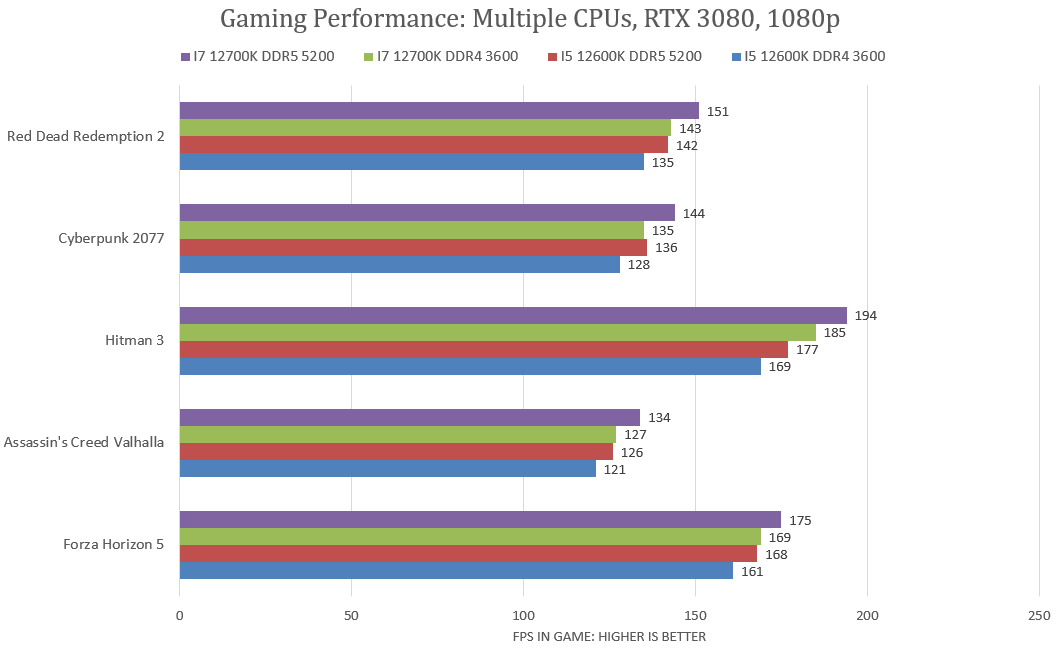
\includegraphics[width=13cm]{figures/Diagram Gaming Performance Multiple CPUs.png}
    \caption{Average performance with Intel Core i5 12600K and i7 12700K \parencite{youtube_test_i7+i5, youtube_test_i5}}
\end{figure}

As we can see in Figure 1, there are minor changes between the use of DDR4 and DDR5 inside a CPU configuration. We also see that at most of the games, the weaker i5 12600K with DDR5 RAM can on average compete with the stronger i7 12700K with DDR4 RAM. On average, the i5 12600K with DDR5 even beat the i7 12700k with DDR4 in Cyberpunk 2077 \parencite{youtube_test_i7+i5, youtube_test_i5}.
\\
We also wanted to know how much of a difference the RAM can make at only one CPU. That is why we searched for tests only regarding the Intel Core i9 12900K, the best CPU of Intel's 12th generation line-up. For these tests, two different RAM modules for each generation were used to see how much of a difference even inside a DDR generation it can make. The RAM that was used are DDR4 at 3200 MHz with a CAS latency of CL14 and 4000 MHz with a CAS latency of CL14, while the DDR5 modules are clocked at 4800 MHz and 6000 MHz and at CAS latencies of both CL36. The GPU that was used in these tests is an AMD Radeon RX 6900 XT, while the screen resolution stays the same as in the test of Figure 1.

\begin{figure}[H]
    \centering
    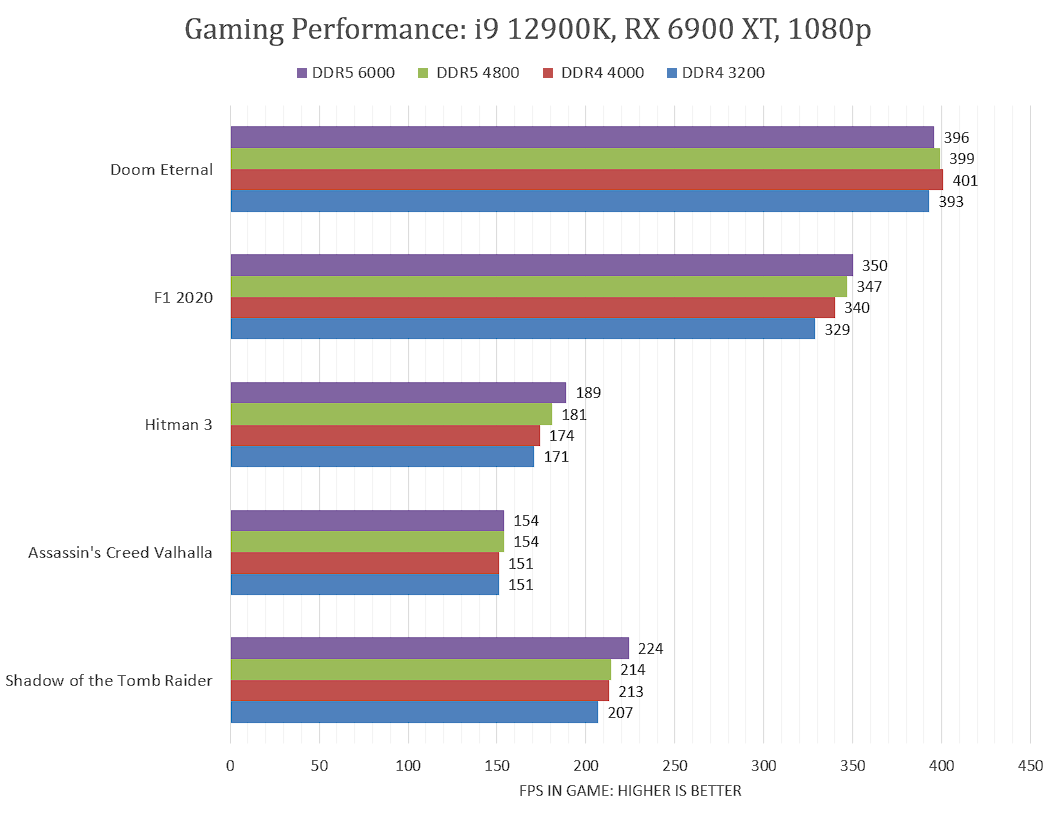
\includegraphics[width=13cm]{figures/Diagram Gaming Performance i9.png}
    \caption{Performance with Intel Core i9 12900K \parencite{12900k_gaming_and_work_benchmarks}}
\end{figure}

We can see in Figure 2, that with every RAM change, there is also an improvement in performance. What is a bit surprising, is that DOOM Eternal runs better at DDR4 RAM with a clock speed of 4000 MHz than DDR5 RAM as a whole \parencite{12900k_gaming_and_work_benchmarks}.
\\
\\
Because the gaming performance draws not the whole picture, we also took a look at synthetic benchmarks. In these benchmarks, only an Intel Core i9 12900K was used. Figure 3 shows the results of 3DMark. Here, 4 different RAM kits that were used, two kits for each generation.

\begin{figure}[H]
    \centering
    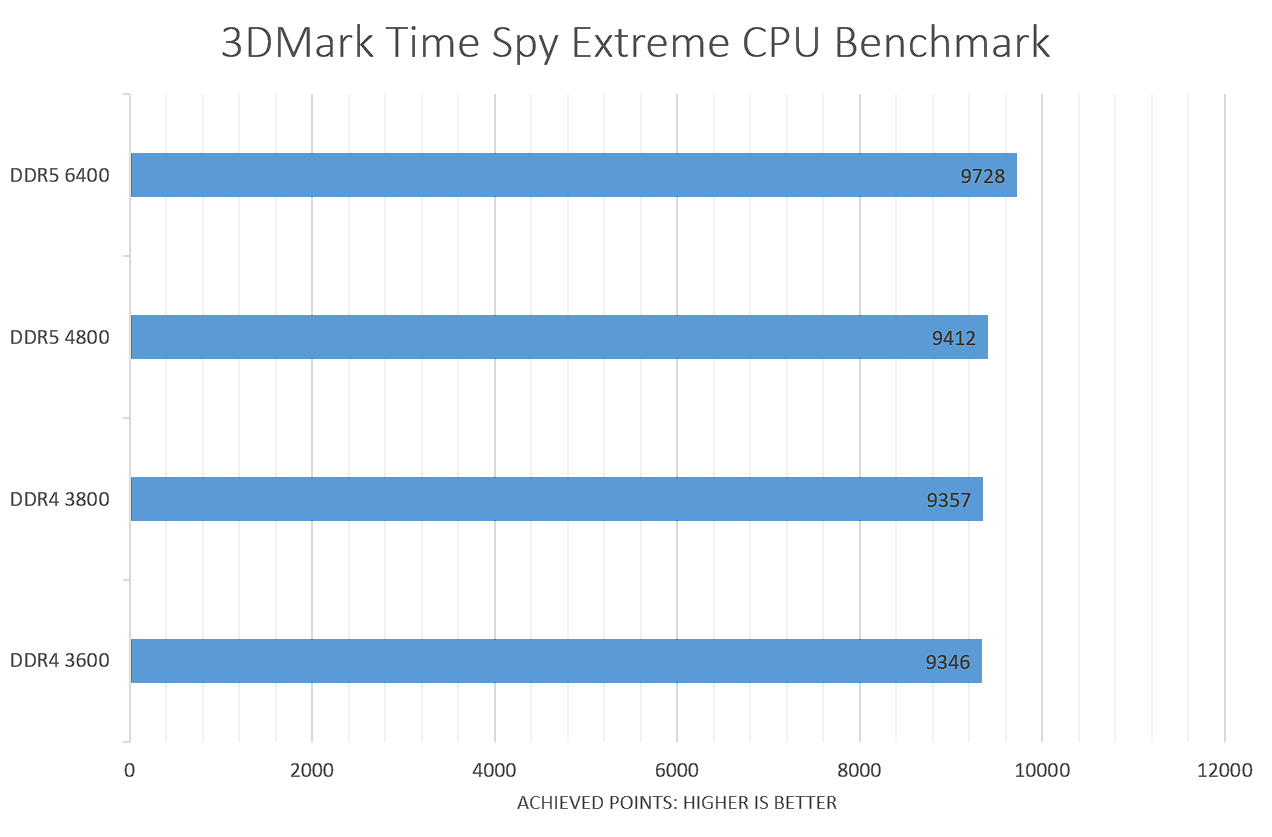
\includegraphics[width=13cm]{figures/Diagram 3DMark.png}
    \caption{Performance of i9 12900K in a general stress test \parencite{youtube_test_3dmark}}
\end{figure}

The RAM kits that were used are two DDR4 and two DDR5 kits. The DDR4 kits are having a frequency of 3600 MHz and 3800 MHz while both having a CAS latency of CL16, while the DDR5 kits are having a frequency of 4800 MHz and 6400 MHz and a CAS latency of CL40 for the 4800 MHz kit and CL38 for the 6400 MHz. As we have seen in the gaming comparison, each RAM step up again provides a small performance improvement, which is around 1\% - 4\% for each RAM step up. That means that the CPU can perform in a general stress test around 2\% - 3\% better when a fast DDR5 kit is used \parencite{youtube_test_3dmark}.
\\
\\
For a more specific test, the compressing and decompressing files with the 7-Zip application, the Intel Core i9 12900K was paired with a DDR4 kit with a frequency of 3600 MHz at a CAS latency of CL16 and a DDR5 kit with a frequency of 5200 MHz at a CAS latency of CL40. Figure 4 shows the compressing and decompressing rate in \gls{MB/s} of both tests.

\begin{figure}[H]
    \centering
    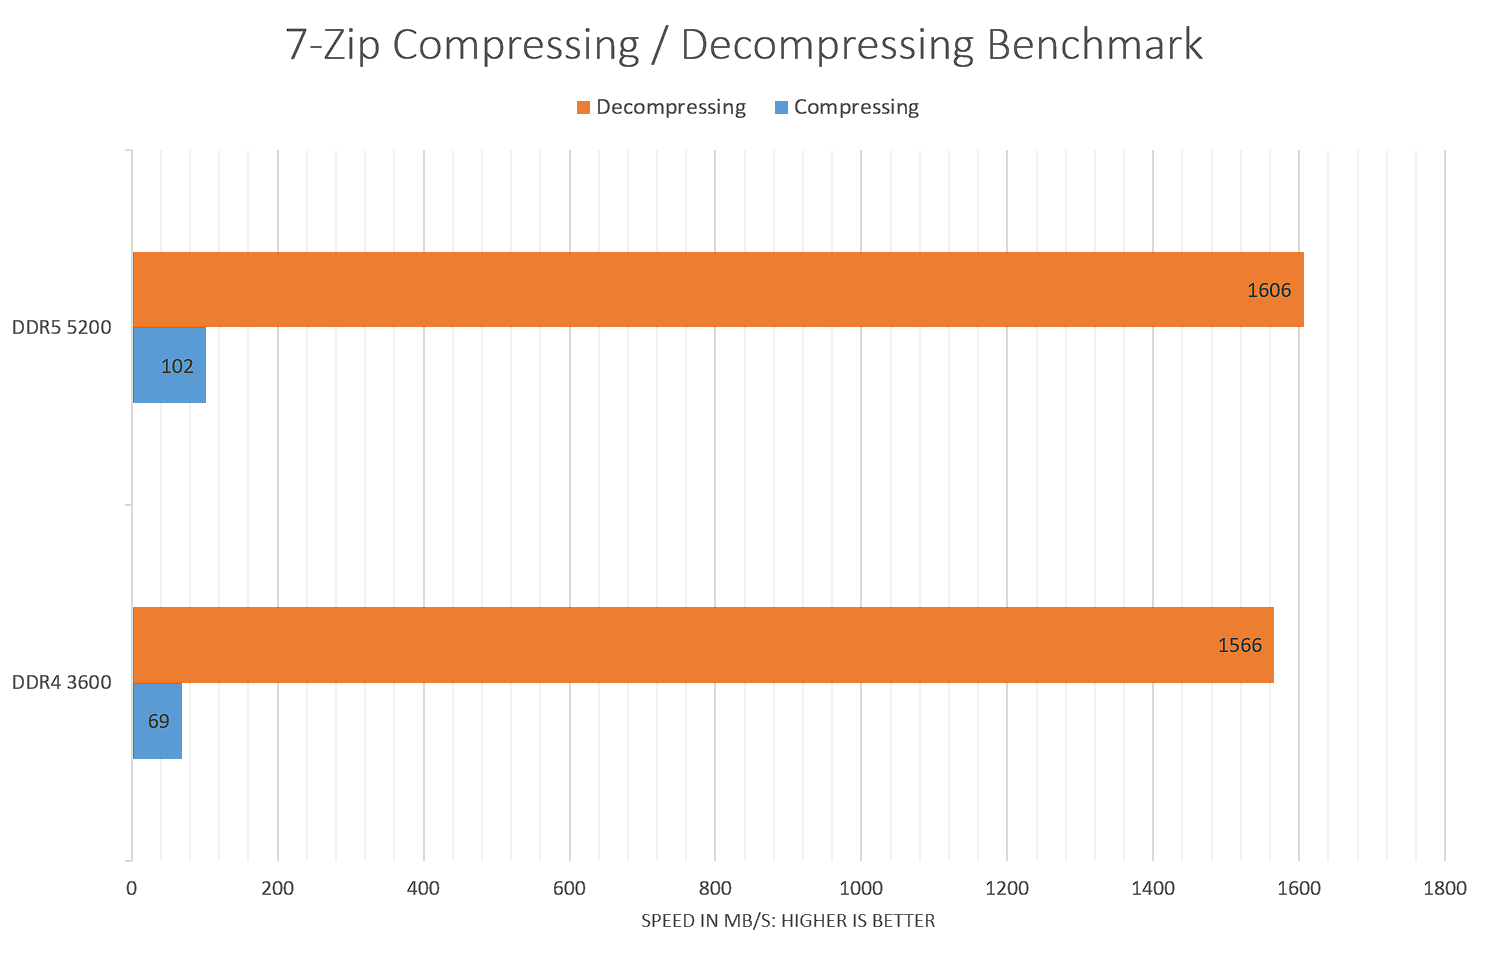
\includegraphics[width=13cm]{figures/Diagram 7-Zip.png}
    \caption{Compression and decompression test with 7-Zip \parencite{test_7zip}}
\end{figure}

As we can see in Figure 4, the tests show, that the CPU can perform around 45\% faster at compressing files when using the DDR5 kit, while performing around 3\% faster at decompressing files when using the DDR5 kit. This test respectively shows, when using DDR5 RAM, that the CPU is performing a bit faster in multithreaded workloads \parencite{test_7zip}.
\\
\\
Because these tests did not test for any creative work, we also included a test that benchmarks the performance of the system in Adobe Photoshop. This tool is called PugetBench, and it tests the encoding strength of the CPU, which is important for creative work like Adobe Photoshop or streaming on streaming services like Twitch \parencite{what_is_pugetbench}. For the tests, again an Intel Core i9 12900K with two RAM kits were used, one DDR4 kit at a frequency of 3200 MHz at a CAS latency of CL22, while the DDR5 kit runs at a frequency of 4400 MHz at a CAS latency of CL40. Figure 5 shows the results of said tests.

\begin{figure}[H]
    \centering
    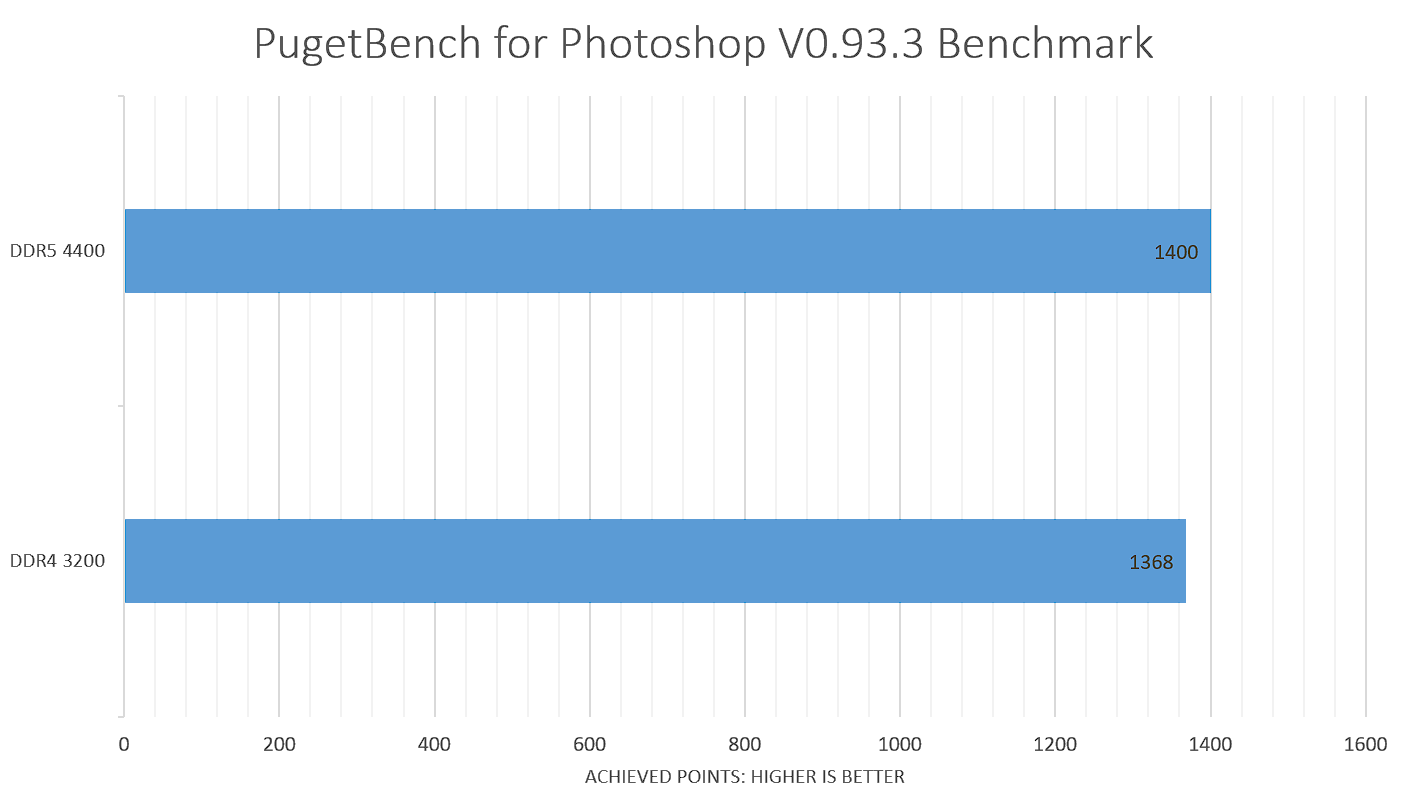
\includegraphics[width=13cm]{figures/Diagram PugetBench.png}
    \caption{Performance of i9 12900K in creative work \parencite{pugetbench_test}}
\end{figure}

Again, we can see a small 3\% increase in performance when using the DDR5 RAM kit. This means that if someone uses creative apps, like Adobe Photoshop or Blender, or is streaming on Twitch or another streaming platform, DDR5 can improve the performance a bit \parencite{pugetbench_test}.
\\
To conclude, when using DDR5, a mostly small improvement (1\% - 45\%) can be expected across the CPU.

\newpage

\subsection{Price-performance Comparison}

Now that we know the performance difference, we want to know if the price of DDR5 is changing over the year. Because DDR5 was firstly introduced at the end of 2021, there is not many data that can be used to define the price of that time. That is why Figure 6 shows the price of DDR5 only from March. The prices that are compared in Figure 6 are from RAM kits from the manufacturer Crucial. The first RAM kit is a 2 × 16 GB DDR4 RAM kit running at a frequency of 3200 MHz at a CAS latency of CL20, while the second RAM kit is a 2 × 16 GB DDR5 RAM kit running at a frequency of 4800 MHz at a CAS latency of CL40. Even though the retail price of the DDR4 kit is set at a price of €103.52 \parencite{Crucial_ddr4} and the DDR5 kit is set at a price of €148.74 \parencite{Crucial_ddr5}, vendors set their prices to how demanded the kits are.

\begin{figure}[H]
    \centering
    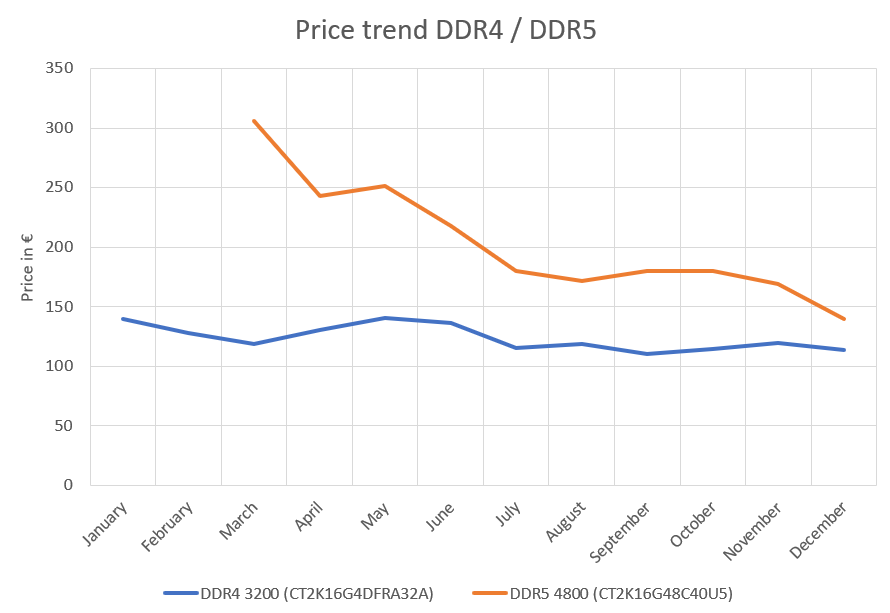
\includegraphics[width=13cm]{figures/Diagram Price Trend.png}
    \caption{Price trend of DDR4 kit and DDR5 kit in 2022 \parencite{Geizhals_ddr4, Geizhals_ddr5}}
\end{figure}

We see that DDR5 was at the beginning of 2022 very expensive. We also see, that the price for DDR5 has fallen, and at the end of 2022, the DDR5 kit costs half of what it would cost in March. These price changes did not affect the price trend of the DDR4 kit at all. It can be seen, that the price for the DDR4 kit did not change dramatically, like how the price of the DDR5 kit did. Still, the DDR5 kit costs around 16\% more than the DDR4 kit at the end of the year.
\\
\\
Performance and price are two separate categories, which have nothing to do with each other. However, with calculations, a connection between price and performance can be established. This helps to evaluate, if a specific configuration is worth the additional costs. In Table 2, we included first the average price of every kit that was used in the tests above. The rest data conclude how much performance someone per Euro in the tests above would get. As we can see in Table 2, the price-performance ratio is with DDR4 in almost every category higher than it is with DDR5, except in the 7-Zip Compress benchmark. Here, DDR5 provides a tiny bit more performance per Euro than DDR4. What this all means will be discussed in the next chapter. 

\begin{table}[H] 
    \centering
    \begin{tabular}{|m{5cm}|P{3cm}|P{3cm}|}
    \hline
                                             & \textbf{DDR4}  & \textbf{DDR5}    \\ \hline
    Average cost per used kit (Euro)         & 107,75         & 159,11           \\ \hline
    Games (FPS)                              & 3,715          & 1,306            \\ \hline
    3DMark (Points)                          & 86,789         & 60,147           \\ \hline
    7-Zip Decompress (MB/s)                  & 14,534         & 10,094           \\ \hline
    7-Zip Compress (MB/s)                    & 0,64           & 0,641            \\ \hline
    PugetBench (Points)                      & 12,696         & 8,799            \\ \hline
    
    \end{tabular}
    \caption{Performance per Euro ratio}
\end{table}
\section{Discussion}

This chapter will discuss all the found results that were shown in the previous chapter. This chapter will also answer our research question and our hypothesis.

\subsection{Architectural Discussion}

As we have seen in Table 1, there were a lot of architectural changes with DDR5. DDR5 is way faster while consuming 10\% less power. This probably will not affect the power consumption of a PC as a whole dramatically, but it can save unnecessary power output on laptops, that are dependent on a battery that lasts a long time. As it was with DDR3 to DDR4, the laptop industry might consider changing to DDR5 where it is possible to save that power. In addition to the less power consumption, the PMIC, that was on the motherboard the generations before, is now soldered onto the module itself. This allows the modules to operate at 1.1 \gls{V} due to better power management, while also reducing potential noise \parencite{ddr5_overview_kingston}.
\\
\\
The chip density also got a huge boost. Now, one single chip on the module can contain up to 64 GB of data. This will mostly affect data centres, as they need high capacity RAM for their servers. Samsung even announced, that with DDR5, it is possible for them to create a module that can contain 1 \gls{TB} \parencite{samsung_1tb}. If these excessive amounts of capacity, that are possible with DDR5, will also be available for the normal PC user, cannot be said confidently.
\\
\\
What is surprising, is that the latencies and CAS latencies are much higher with DDR5 than it was with DDR4. CAS latencies determine how many clock cycles happen to put data from the CPU onto the RAM module, so it can be read again. However, the latency, which is given in \gls{ns}, determines how long the delay is between a data request from the CPU and when the data at the CPU arrives \parencite{DDR4_DDR5_CAS}. The CAS latency is much higher than it was with DDR4, but it does not explain everything related to latency. As we can see, the latency in ns has also increased with DDR5, but not as much as it could be expected considering the increase of the CAS latency. Because of this and the much higher data rate, the higher latencies are not affecting the performance by making the RAM less responsive \parencite{RAM_Latency}.
\\
\\
What could be an influence to the higher latencies, are the reliability changes, that were made. As we already disclosed, the CRC, which checks for invalid data that is being inputted to the RAM chip \parencite{crc_def}, has been introduced to the read cycle of the module. Now, DDR5 performs a CRC check with every cycle, regardless if it is a read or a write cycle. Also, On-Die ECC was introduced to every DDR5 RAM module. While the CRC checks, if the data that are inputted or outputted are correct, On-Die ECC can correct incorrect or damaged data \parencite{ddr5_overview_kingston}. Before, ECC was only reserved for special ECC RAM, that was exclusively used in servers. Now with DDR5, every module gets On-Die ECC correction. These changes improve the reliability of data, but it is unlikely to make a difference in daily usage. This is because even with DDR4, the only errors that result in blue screens that can happen on Windows related to RAM are about broken RAM modules or misconfigured power management for the RAM modules, and not incorrect data \parencite{bluescreens}. 
\\
\\
As the last changes, the Bank Groups of each module have increased to 8 groups, while keeping the Banks per Group the same. A bank in a RAM chip is a field, that contains the stored data, while a bank group is a package that contains these fields. Each bank group transfers data to the CPU one at a time. Banks need to recover by “refilling” with data, before they can transfer data again \parencite{bank_groups}. With the high data rate that comes with DDR5, this can be a problem, because how can a bank group transfer data to the CPU, when the banks are not recovered yet? To accommodate this, the number of bank groups have been increased to 8. In addition to that, the channel that is used to transfer data to the CPU has been split up from a single 64 bit channel to a dual 32 bit channel. This is again improving latency and efficiency, because we have now two independently working channels, that have lower bits needed to transfer to the CPU \parencite{ddr5_overview_kingston}.
\\
\\
All these changes can improve system stability, which is mostly important in server applications. For a home PC user, the higher data rate and the lower power consumption are probably the most important changes. The other changes will not have a noticeable effect on the system of a home PC user, other than better performance.

\subsection{Performance Discussion}

The architectural changes contributed to a small performance boost across the CPU. 
\\
As we can see in Figures 1 and 2, when using the DDR5 kits, the system performs on average 5\% better both the multiple CPU test and the single CPU test. The only exception are the results in the DOOM Eternal test in Figure 2. Here, DDR4 performs better than DDR5. Again, we cannot check if this is true or an error in the test, because we cannot test these results by ourselves. For the other test results, it can be a decent upgrade to use DDR5 RAM instead of DDR4. When we take a look at Figure 1, we see that the i5 12600K can compete with the much stronger i7 12700K when using a DDR5 RAM kit. The i5 12600K even beat the i7 12700K on average FPS in Cyberpunk 2077. 
\\
Generally speaking, a 5\% performance boost in games can be expected when using DDR5 instead of DDR4.
\\
\\
When we now look at the performance graphs of the synthetic benchmarks, we also see, that DDR5 performs better. However, here are the differences not that clear like in the game benchmarks. The 3DMark test in Figure 3 shows that the CPUs performance improve as a whole when using especially fast RAM, because there is an around 300 Points jump between the 6400 MT/s RAM and the 4800 MT/s RAM. When we take a look at the PugetBench results in Figure 5, we see that the CPU performs around 2\% better. The 7-Zip test in Figure 4 is more interesting. The decompressing rate has increased by 2\%, while when we look at the compressing rate, we see that the CPU performs around 48\% better when using DDR5. That means that the CPU performs a bit better when using work applications like Photoshop, encoding videos for streaming or other creative work, while performing much better in handling files. 
\\
\\
This is also the reason we need to use tests for both gaming and work performance. Just looking at the graphs, of course it can be seen that DDR5 performs better than DDR4, but just from the gaming benchmarks, we cannot conclude how much better DDR5 performs in work applications. Gaming benchmarks only test for the gaming capabilities, without stressing the system hard enough to get a better insight of how well the system will perform in creative work or other applications. The same can be said the other way around. Just because we see a 48\% improvement in the compressing file benchmark, does not necessarily mean that our gaming performance also will increase that much. So it is always necessary to test for both gaming and work performance.

\subsection{Price-performance Discussion}

While there is an improvement in performance, we also need to check if the price-performance ratio is acceptable to answer our research question. As we can see in Table 2, the price-performance ratio is not speaking for DDR5. In the benchmarks, DDR4 performs with a better price-performance ratio, giving more performance per Euro spend. In Figure 6, we have also compared two RAM kits from the manufacturer Crucial, and we discovered that the DDR5 kit is around 16\% higher priced than the DDR4 kit. However, this does not compare to the average costs of the kits that were used for the benchmarks. As Table 2 shows, the average DDR4 kit in the benchmarks costs €107.75, while the average DDR5 kit costs €159.11 \parencite{used_kits}. 
\\
\\
We also do need to remember, that with DDR5, a new motherboard needs to be purchased, because DDR4 and DDR5 does not have the same socket. This will also increase the price that needs to be spent for DDR5. This also speaks, from a cost perspective, more for DDR4, if DDR4 is already in use.

\subsection{Conclusion}

To conclude, DDR5 is a small improvement in gaming performance, and depending on the use case, a bigger performance in work applications. 
We can answer our research question with “DDR5 provides a small performance in gaming and work applications over DDR5”. However, we cannot confirm our hypothesis, because we hypothetized that DDR5 also provides a better price-performance ratio, which it did not. If now someone is in a situation, where they want to upgrade their PC system, we probably would not recommend upgrading to DDR5 RAM, because from our perspective, it is not worth it to spend over €130 plus a new, most likely expensive motherboard for a small improvement. However, as DDR4 replaced DDR3, DDR5 will be the new RAM standard that more and more new CPUs will only be compatible with, as it is already with the new AMD Ryzen 7000 series is \parencite{Ryzen_7000_RAM_specs}. It also could be, because the technology is still pretty new, that it will be improved over the years to be more attractive than DDR4, but from today's perspective, we would not recommend upgrading to it, if that was our research topic.

\subsection{Further Research}

As we already have disclosed multiple times already in this report, the main problem was that we could not do the tests ourselves. This is because we did not have the necessary hardware, more specifically the latest CPUs of Intel and DDR5 RAM. To make this report more reliable and to improve the results of this report, the necessary hardware would be needed. 

\printbibliography[title=References]

\end{document}